\section{Checkpoint 3 - Branch Predictor}
In our current datapath design, we handle data hazards by forwarding path, but we do not handle control hazards well. This results in high CPI as our naive predictor (always predict non-taken) often mispredict and we need to stall or flush the pipeline upon such misses. 

In Checkpoint 3, we want to explore the idea of a \textbf{Branch Predictor}. This particular predictor should predict the direction of branch (whether it is taken or not), not the address of branch target. There are many ways to implement branch predictors, but for consistency of this checkpoint please follow the scheme we describe below as you need to pass our testbench. You can build a better and more sophisticated branch predictor in Checkpoint 4 Optimization. 

\subsection{Branch History Table Overview}
Branch History Table (BHT) or Branch-Prediction Buffer (BPB) is a form of dynamic branch prediction, which allows our prediction to adapt to program behavior.  

To do so, we need to build the branch predictor that can 
\begin{itemize}
    \item \textbf{Guess:} When the branch instruction is in the first stage of processor, make a prediction whether to take the branch based on the past history.
    \item \textbf{Check:} When the branch instruction reaches the second stage of processor (where branch result is resolved), check if your prediction is correct and update to make better prediction next time.
\end{itemize}

One way to build such a system is by building a \textbf{cache} whose entries that is represented by a \textbf{saturating counter}. 

\textbf{2-bit Saturating Counter} is a state machine that correspond to a particular branch instruction (based on its address) to show whether the branch was recently taken or not. We can use that information to make a prediction as past is usually a good indicator of the future. We increment the counter on branch taken and decrement it on branch not taken. Instead of a single bit that represents taken or not taken recently, we make it more robust by using two bits and less sensitive to anomaly branch behaviors. We can take the top bit as the prediction. For example, if the branch behavior is mostly not taken and the state is currently in strong not taken, even the branch is taken once, it will still be weakly not taken and prediction remains not taken. 

\begin{figure}[hbt]
\begin{center}
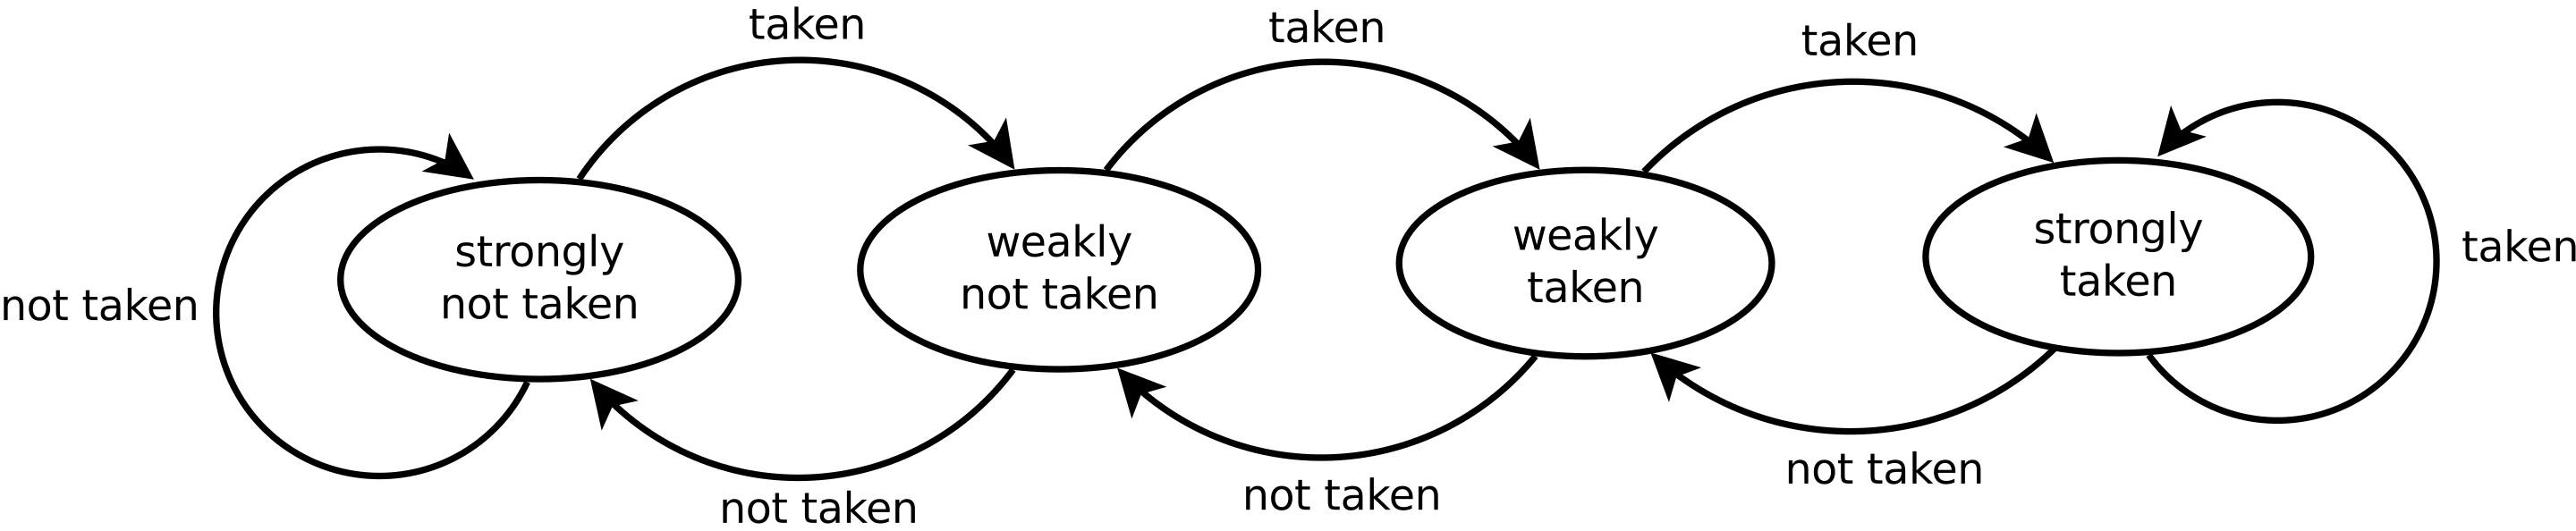
\includegraphics[width=0.9\textwidth]{figs/saturating_counter.png}

\caption{State Machine for 2-bit Saturating Counter.}
\end{center}
\end{figure}


\newpage
\textbf{BHT / BPB as a Cache}. The branch history table and branch prediction table can be thought of a cache or a buffer. We map each branch instruction by the lower portion of the address into entries of the cache (index into cache by lower address bits). Each cache line contains the saturating counter value that represents history of the instruction. During the guess stage, we check if the cache contains entries of this branch instruction by checking the tag and valid bit. If it is a hit, we read the entry and use the top bit as prediction. 

During the check stage, we read the entry of the cache again to see if behavior of corresponding branch instruction has been recorded. If the entry exists (cache hit) we read and update the current saturating counter based on whether the branch is taken or not, and write back to the cache with updated saturating counter value. If the entry did not exist before, we write a new line in the cache with saturating counter value based on whether the branch was taken or not.


\begin{figure}[hbt]
  \begin{center}
    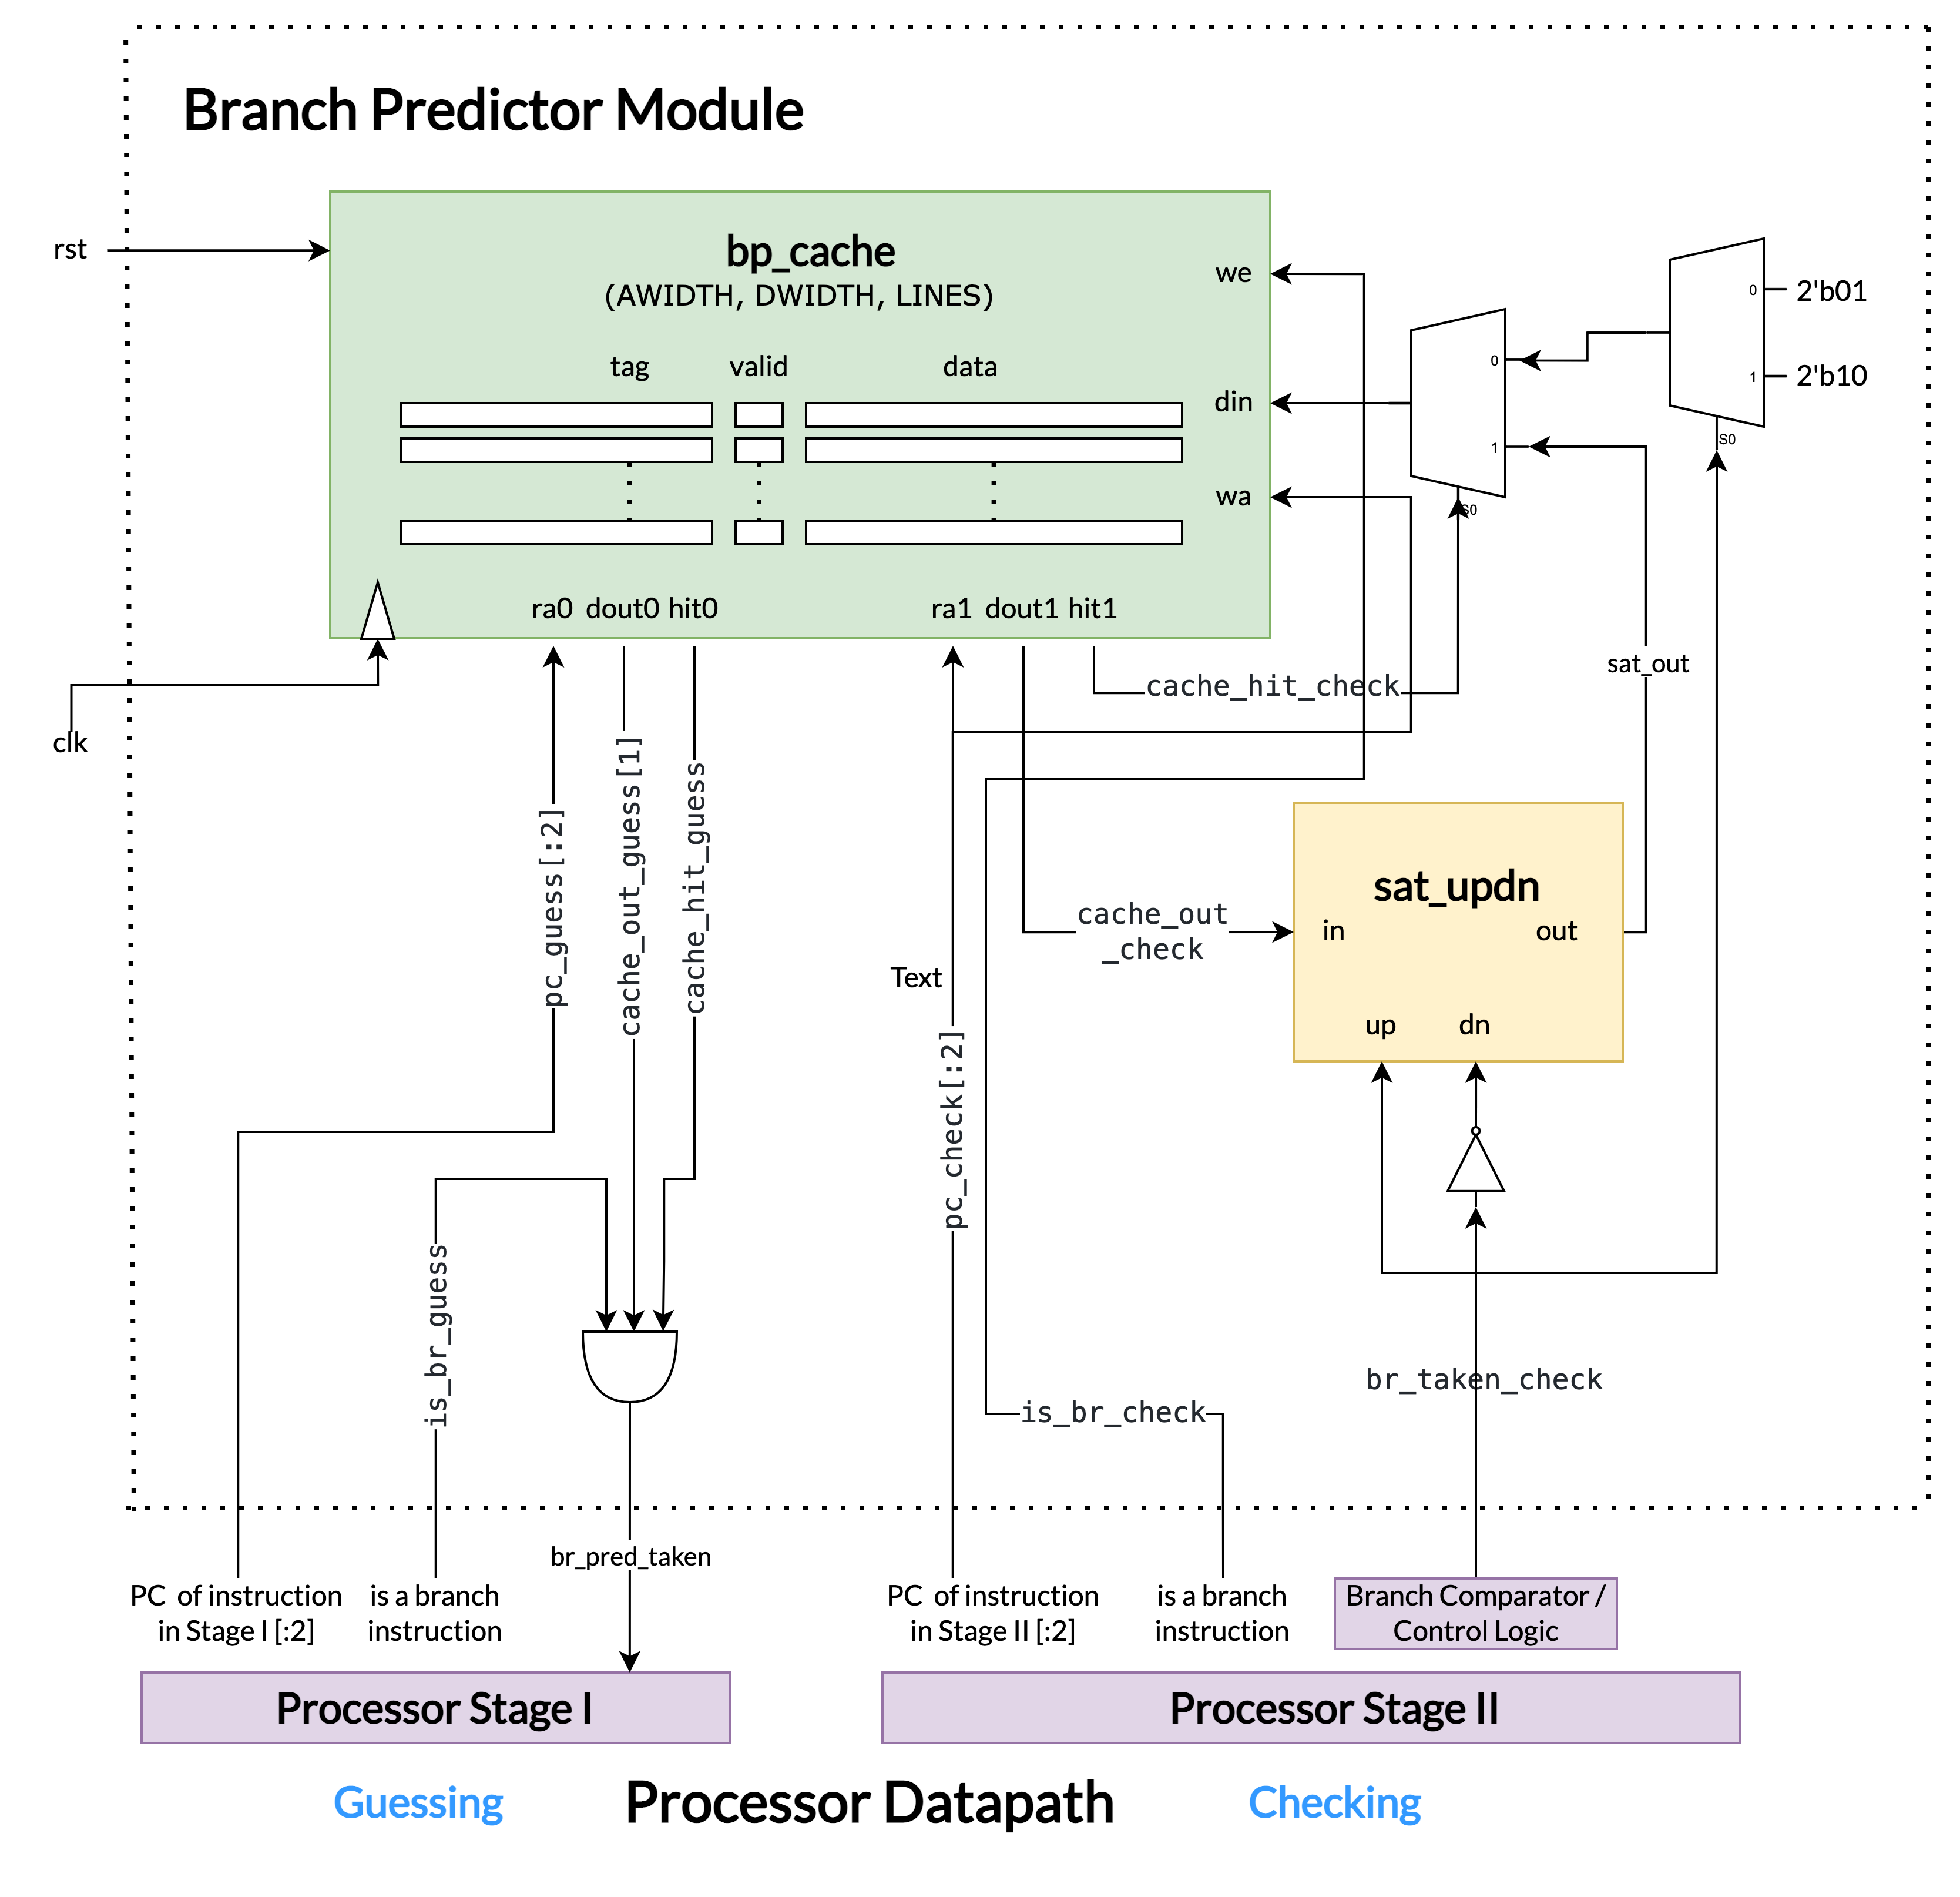
\includegraphics[width=0.9\textwidth]{figs/branch_predictor.png}
    \caption{Structure of the Branch Predictor Module; see how the cache, saturating counter composes the branch predictor and how it interacts with signals from Stage I and II of the processor datapath.}
  \end{center}
\end{figure}


This formulation treats the BHT just as a regular cache, but with entry that represents a saturating counter which can be used for branch prediction. The diagram below illustrates the module interface our skeleton code provide. We separate the module into a cache and a saturating counter. The cache supports 2 asynchronous reads as we can simultaneously have two branch instructions in flight in Stage I and II. The cache supports 1 synchronous write to update its entry. 

\subsection{Guidelines and requirements}
Please pull the skeleton again before starting this checkpoint. We have added skeleton code in  hardware/src/riscv\_core/branch\_prediction as well as test benches and modifications to other parts of the datapath and software to support adding the branch predictor. Before you start this, make sure you have Checkpoint 2 datapath implemented with naive branch predictor and have mechanism to recover from branch mispredict, as we will solely be replacing naive predictor with a more accurate one.

\begin{enumerate}
  \item Within hardware/src/riscv\_core/branch\_prediction, we have prepared branch\_predictor.v which is the top level branch predictor. It uses components bp\_cache.v and sat\_updn.v which for both you would implement. You do not need to modify branch\_predictor.v. It is important to understand how they all interface with each other, and how you can instantiate and connect the branch\_predictor in your datapath.
  \item Implement a 2-bit \textbf{saturating counter} in sat\_updn.v. Note this should be a purely combination circuit that takes in existing counter value and whether to increment/decrement and compute the new counter value. We do not provide a test bench but we recommend you write one.
  \item Implement the \textbf{cache} in bp\_cache.v, with 2 asynchronous read ports and 1 synchronous write port. Each cache line has tag, valid bit, and fields to store the data. The cache should be parameterizable by address width, data width, and number of cache lines.
  \begin{enumerate}
      \item EECS151 Student should implement a \textbf{direct-mapped} cache.
      \item EECS251A Student should implement either 1) a direct-map and a 2-way set associative cache. 2) a configurable N-way set associative cache. 
    \end{enumerate}
   We will not be providing a test bench for the cache. However, you are \textbf{required} to design a test bench for your cache that covers representative cases such as read miss, read hit, write, eviction, etc (251 students to write test regarding the associativity). You will need to \textbf{explain} your cache testbench to a TA upon checkoff. 
  \item With both saturating counter and cache implemented, you have completed the branch predictor module. We have provided a \textbf{testbench} in hardware/sim/branch\_predictor\_tb.v. You branch predictor must \textbf{satisfy} the behavior of this test bench for this checkpoint!
  
  \textit{Note for 251A students:} The final test case in branch\_predictor\_tb tests cache hit/miss after cache line replacement \textbf{assuming a direct-mapped cache}. You will need to update this test case to deal with a 2-way set associative or a configurable N-way set associative cache.
  \item Connect the branch predictor module to the rest of your CPU datapath, with inputs and output in appropriate stages of your CPU (this will vary based on your design). Make sure you still pass all the checkpoint 2 tests so it is still functionally correct. 
  \item To track performance of your branch predictor, we ask you to add two counters, one for \textbf{total} number of branch instructions the CPU encountered, and one for the number of \textbf{correct} predictions. These counters should be mapped as \textbf{Memory Mapped IO} to address 0x8000\_001c and 0x8000\_0020 respectively; they can also be reset similar to cycle and instruction counters. See 2.9.4 Memory Mapped I/O section for updated mapping.  With these stats, you can calculate the \textbf{branch prediction accuracy}. The mmult program has been modified to print those results at the end as well, make sure you recompile it after pulling the changes. 

  We have also provided a testbench in hardware/sim/mmio\_counter\_tb.v, which will run a small set of instructions and print out the MMIO counter values. You may find it helpful to debug branch prediction and MMIO counters here in simulation before testing it on the FPGA. Feel free to add additional test cases.
  \item We connected SWITCH[0] to enable bp\_enable. Once you successfully uploaded the new design to CPU, run mmult with the switch off and on will show the result with branch prediction off / on. The checksum should remain the same but you should see improved performance with branch prediction enabled.
  
\end{enumerate}

\subsection{Checkoff}
\textbf{\branchPredictorTaskName \space materials should be committed to your project repository by \branchPredictorDueDate.}

\begin{itemize}
    \item Pass test bench in hardware/sim/branch\_predictor\_tb.v
    \item Explain your cache test bench design and how that covers all the representative scenarios for your cache to the TA.
    \item Run mmult with branch prediction disabled and enabled by toggling the switch. The program must still be functionally correct with the correct checksum. For both settings, record the CPI, the amount of total branch predictions, the amount of correct branch predictions, and calculate branch prediction accuracy. CPI and branch prediction accuracy must be \textbf{strictly better} with Checkpoint 3 branch predictor pass this checkpoint.
\end{itemize}

\newpage
